\documentclass[a4paper,12pt]{article}
\usepackage[utf8]{inputenc}
\usepackage{graphicx}
\usepackage[affil-it]{authblk}
\graphicspath{{images/}}
\usepackage{listings}
\usepackage{indentfirst}
\usepackage{varwidth}
\setlength{\parskip}{10pt}

\begin{document}

	\begin{titlepage}
		\begin{center}
			\textbf{\huge Layered Architecture}
			
			\vspace{0.5cm}
			
			{\large Software Architecture}
			
			\vspace{1.5cm}
			
			
\includegraphics[width=0.7\textwidth]{Pradita Logo.png}
			
			\vspace{1.5cm}
			
			\textbf{\large Disusun oleh:}
			
			\vspace{0.5cm}
			
			\begin{varwidth}{\textwidth}
				\begin{itemize}
					\item Muhammad (2110101031)
					\item Austin Nicholas T. (2110101003)
					\item Darren Valentio (2110101009)
				\end{itemize}
			\end{varwidth}
		
			\vspace{3.5cm}
			
			\textbf{\large TEKNIK INFORMATIKA}
			
			\vspace{0.5cm}
			
			\textbf{\large PRADITA UNIVERSITY}
			
			\vspace{0.5cm}
			
			\textbf{\large 2023}
		\end{center}
	\end{titlepage}

	\section*{Definisi \textit{Layered Architechture}}
	
	Pola arsitektur layered adalah pola n-tiered di mana komponen disusun dalam lapisan horizontal. Ini adalah metode tradisional untuk merancang sebagian besar perangkat lunak dan dimaksudkan untuk pengembangan mandiri sehingga semua komponen saling berhubungan tetapi tidak saling bergantung.
	
	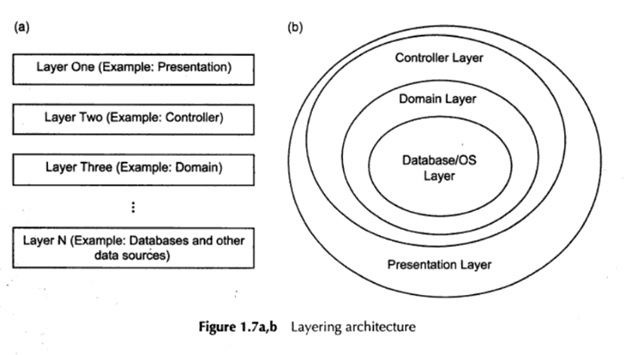
\includegraphics{Layering Architecture.jpg}
	
	Seperti yang ditunjukkan pada gambar, layering biasanya dilakukan dengan mengemas fungsionalitas khusus aplikasi di lapisan atas, penyebaran fungsionalitas spesifik menjadi lapisan bawah dan fungsionalitas yang membentang di seluruh domain aplikasi di lapisan tengah. Jumlah lapisan dan bagaimana lapisan-lapisan ini disusun ditentukan oleh kompleksitas masalah dan solusinya.
	
	Di sebagian besar arsitektur berlapis, ada beberapa lapisan (atas ke bawah):
	
	\begin{itemize}
		\item \textbf{The application layered:} Berisi layanan spesifik aplikasi.
		\item \textbf{The business layer:} Menangkap komponen yang umum di beberapa aplikasi.
		\item \textbf{The middleware layer:} Lapisan ini mengemas beberapa fungsi seperti pembangun GUI, antarmuka ke basis data, laporan, dan dll.
		\item \textbf{The database/System Software Layer:} Berisi OS, database, dan antarmuka ke komponen perangkat keras tertentu.
	\end{itemize}

\end{document}